\documentclass[a4paper,oneside]{article}
\usepackage{indentfirst}
\usepackage{graphicx}
\usepackage{listings}
\usepackage{newtxtext,newtxmath}
\usepackage[top=0.7in, bottom=0.7in, left = 0.7in, right = 0.7in]{geometry}
\usepackage{enumitem}
\usepackage{caption}
\setlength{\belowcaptionskip}{-10pt}

%\setlist{nolistsep}
\let\OLDthebibliography\thebibliography
\renewcommand\thebibliography[1]{
  \OLDthebibliography{#1}
  \setlength{\parskip}{0pt}
  \setlength{\itemsep}{0pt plus 0.3ex}
}

\begin{document}
\title{\vspace{-0.7in}Term Project Report\\High-Grade Prostate Cancer Prediction using DNA Methylation Data}
\author{Fawwaz Dzaky Zakiyal (201899213)\\Tanjung Dion (201883621)\\}
\date{Bioinformatics (Fall 2018)}
\maketitle
 
\section{Introduction}
Prostate cancer affects a significant proportion of the male population, but in most cases, the disease is harmless. However, for the small portion of the population with high-grade prostate cancer, the disease can be extremely debilitating, causing painful symptoms and even death \cite{prostate}. Over the past years, rapid advances in sequencing technology have led to The Cancer Genome Atlas (TCGA) project which provides the most comprehensive genomic data for various kinds of cancer. In the previous research, to indicates the classification of patient samples was done by using TCGA Exon expression or SNP datasets. However, the recent study shows that DNA methylation act as better bio-markers and help in improving the cancer prognosis \cite{dnameth}. Beside that, in the recent years, machine learning become a useful tool for prediction and regression tasks. It could bring benefit to the cancer risk prediction. Thus, this project implements machine learning techniques to classify high-grade prostate cancer risk using DNA methylation data.


\section{Methodology}
\subsection{Concepts}
\begin{itemize}
\item \textbf{DNA methylation}: the process of adding methyl groups to DNA, in this process modification of covalent nucleotides in the human genome, namely cytosine and also guanine. It is one of epigenetic modification which takes an important role in the development of cancer.
\item \textbf{Gleason Score}: a measure (from 2-10) of the aggression of prostate cancer cells based on clinical pathology of prostate tissue \cite{prostate}.
\item \textbf{High-Grade Prostate Cancer (HGPCa)}: A Gleason score from 8-10 is indicative of High-Grade prostate cancer, while scores below 8 are considered not as severe, HGPCa generally results in poor patient outcomes mortality, complications, and long-term disease-free survival) \cite{prostate}.
\item \textbf{Cancer gene catalogue}: a catalogue those genes which contain mutations that have been causally implicated in cancer.
\end{itemize}

\subsection{Dataset}
The dataset comes from the National Cancer Institute GDC Data Portal and can be found online under Project TCGA-PRAD (The Cancer Genome Atlas Prostate Adenocarcinoma) \cite{praddata}. This dataset consists of genomic information and clinical pathology reports belonging to 549 patients who have been diagnosed with prostate cancer. It contains both clinical (recurrence, survival \& treatment resistance) and molecular profiles (Exon (mRNA) expression, DNA methylation, Copy Number Variations (CNV) \& Single Nucleotide Polymorphism (SNP)). The file that we used are:
\begin{itemize}
\item \textbf{PRAD.meth.by\_mean.data}: the mean signal values among each gene corresponding to the patient barcode. The size is 20111 genes x 549 patients (52 MB). This data become our learning features.
\item \textbf{All\_CDEs}: clinical data elements corresponding to the patient barcode. It contains many related information, but we only consider the gleason score to be the class label.
\end{itemize}

\subsection{System Design}
The process consists of preprocessing of TCGA-PRAD dataset, consist of feature selection, missing data imputation \& adding the label. After that, split the dataset into training \& testing data, next we train \& evaluate the classifier models. The system design can be seen in Figure \ref{fig:system_design}. The system specification where this project running on:
\begin{itemize}
\item \textbf{Programming language}: Python
\item \textbf{Support library}: Scikit-Learn \& Pandas
\item \textbf{PC}: Windows 10 64-bit, Intel i5-7500, RAM 4 GB
\end{itemize}

\begin{figure}
  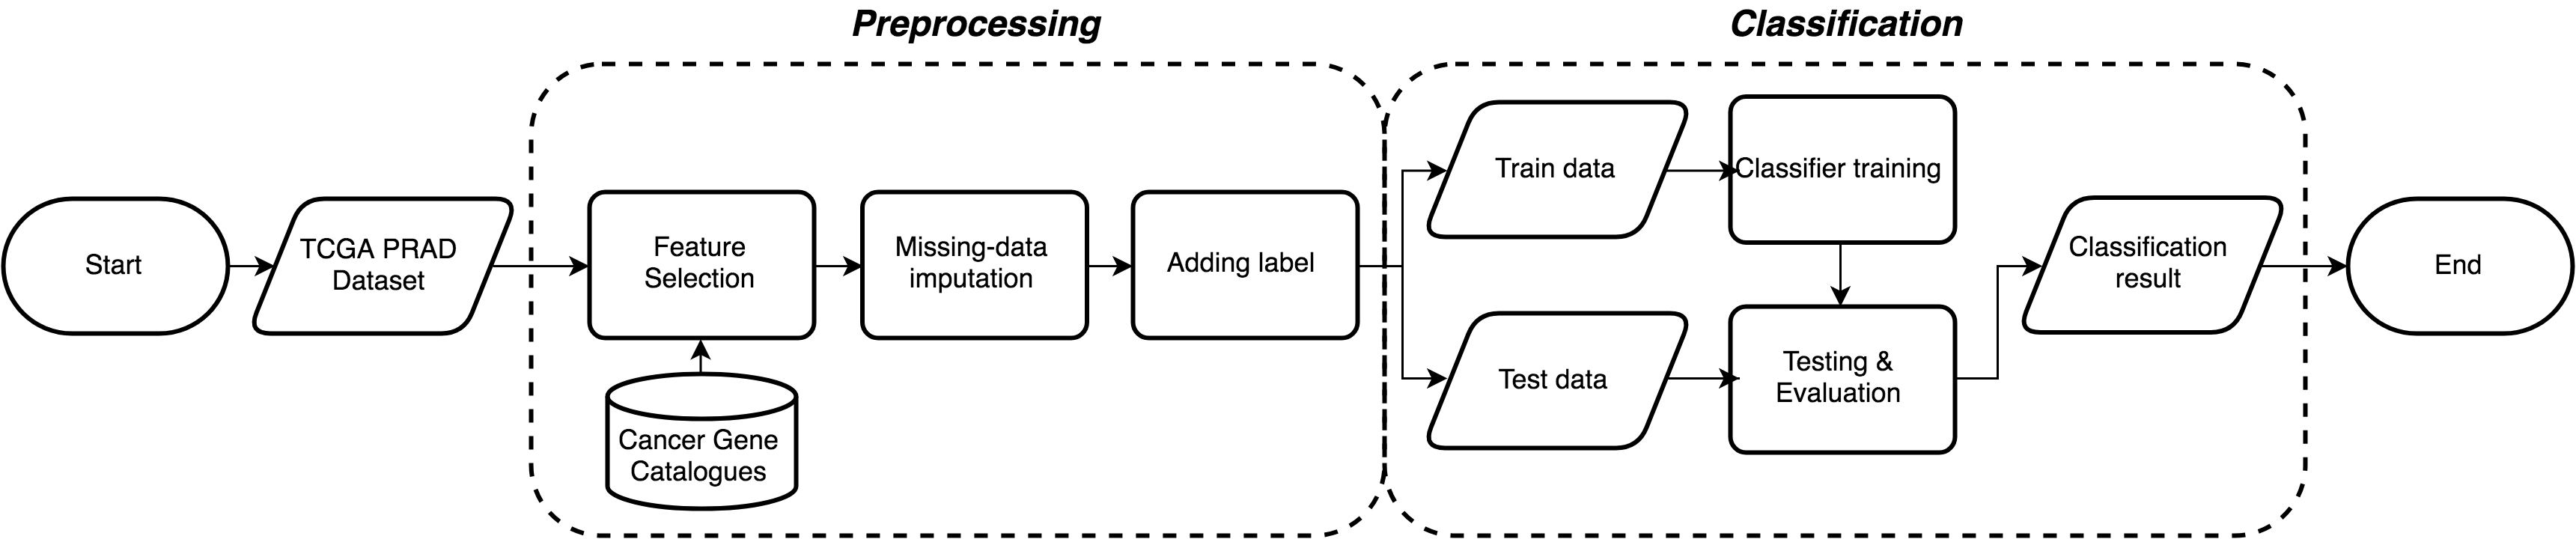
\includegraphics[width=1\linewidth]{system_design}
  \centering
  \caption{System Design}
  \label{fig:system_design}
\end{figure}

\subsection{Preprocessing}
\begin{itemize}
\item \textbf{Feature selection}: To reduce the feature space of the dataset, only those genes for which mutations have been causally implicated in cancer are considered, these are obtained through cancer gene catalogue like \textit{COSMIC} (Catalogue of Somatic Mutations in Cancer) that consist of 3946 genes information \cite{cosmicdata}, and \textit{CIVIC} (Clinical Interpretation of Variants in Cancer) that consist of 366 genes information \cite{civicdata}. Originally, our dataset has 20111 genes, after feature selection it has only 821 genes.
\item \textbf{Missing data imputation}: It is the process of replacing missing data of dataset features with substituted values. This project using mean imputation.
\item \textbf{Adding the label}: We categorized into 2 classes, between score of 2 to 7 (not severe) and 8 to 10 (HGPCa / severe)  from All\_CDEs data. We added class labels to the dataset with correspond to the patient id.

\end{itemize}

\subsection{Classification}
\begin{itemize}
\item \textbf{Dataset split}: We split the dataset, 70\% for train data \& 30\% for test data of each data group (not severe and severe/HGPCa that illustrated in Figure \ref{fig:data_split}.
\begin{figure}
  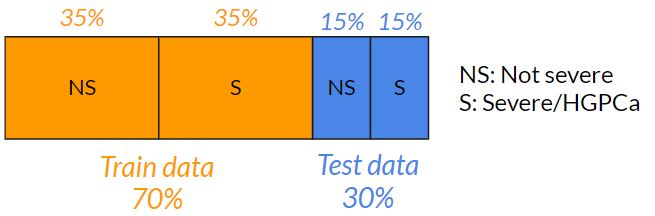
\includegraphics[width=0.4\linewidth]{data_split}
  \centering
  \caption{Dataset split}
  \label{fig:data_split}
\end{figure}
\item \textbf{Training and evaluation}: This project perform on several machine learning algorithms, namely \textit{Logistic Regression}, \textit{K-Nearest Neighbor}, \textit{Support Vector Machine}, \textit{Multilayer Perceptron}. In the experiments, we evaluate parameters for each machine learning method to find the one that gives highest accuracy.
\end{itemize}

\section{Experiments}
\begin{itemize}
\item \textbf{Evaluation on Logistic Regression (LR)}: The experiment cases are LR using L1 or L2 penalty. We fixed the other parameters, such as the regularization parameter \textit{C} (1.0). The result is LR+L1 accuracy (76.36\%) outperform LR+L2. In general, the L1 is expected to be very effective with sparse data, thus it can give a better result. The result shown at Figure \ref{fig:LR}.

\item \textbf{Evaluation on K-Nearest Neighbor (KNN)} : The experiment cases are KNN with number of neighbors 2, 3, 4, or 5. We fixed the other parameters, such as the distance metric (Minkowski). The result is KNN with 3 neighbors accuracy (68.48\%) outperform the other cases. It seems k=3 is the optimum number of neighbors in this experiment. The result shown at Figure \ref{fig:KNN}.

\item \textbf{Evaluation on Support Vector Machine (SVM)}: The experiment cases are SVM using Linear kernel, RBF kernel, or Poly kernel (degree 2, 3, or 4). We fixed the other parameters, such as the regularization parameter \textit{C} (1.0), and the gamma kernel coefficient for RBF \& Poly (1/number of features). The result is SVM using linear kernel accuracy (76.97\%) outperform the other cases that get the same accuracy (61.21\%). It seems that linear kernel get high accuracy indicates the data is linearly separable and the non-linear kernel (RBF \& Poly) low accuracy indicates an over-fitting issue. The result shown at Figure \ref{fig:SVM}.

\item \textbf{Evaluation on Multilayer Perceptron (MLP)}: The experiment cases are MLP using Sigmoid/Logistic, Tanh or ReLU activation function with number of hidden layers 1 (100 neurons) or 2 (100 neurons \& 100 neurons). We fixed the other parameters, such as the optimizer algorithm (Adam), the batch size (200), and the learning rate (0.001). The result is MLP using Tanh activation function with 2 hidden layer accuracy (76.97\%) outperform the other cases. It seems that increasing number of hidden layers lead to increase the accuracy, and generally the Tanh activation function is expected to be very effective with two classes classification task. The result shown at Figure \ref{fig:MLP}.

\end{itemize}


\section{Conclusion}
This project succeeds in implementing machine learning techniques to classify high-grade prostate cancer risk using DNA methylation data. From the experiments, the result shows that SVM and MLP give the highest accuracy at the same value, 76.97\%.
\par
Future work to increase the performance accuracy are further explore in tuning the other parameters of each machine learning algorithms and try in combining the other dataset features, such as SNP, Exon, the other clinical data information (hereditary factors, alcohol consumption, sexual activity, race, etc.).

\begin{figure}[h]
	\centering
	\begin{minipage}[t]{8.6cm}
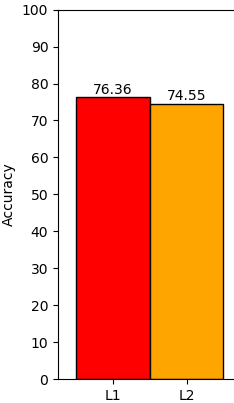
\includegraphics[width=0.4\linewidth]{LR}
  \centering
  \caption{Evaluation on Logistic Regression}
  \label{fig:LR}
	\end{minipage}
	\begin{minipage}[t]{8.6cm}
	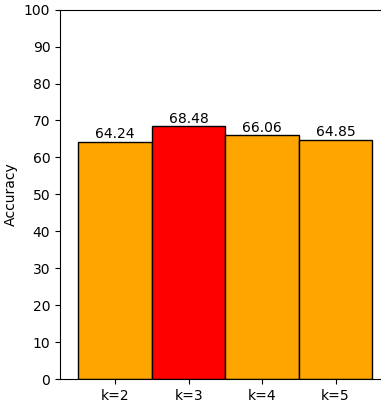
\includegraphics[width=0.65\linewidth]{KNN}
  \centering
  \caption{Evaluation on K-Nearest Neighbor}
  \label{fig:KNN}
	\end{minipage}
\end{figure}

\begin{figure}[h]
	\centering
	\begin{minipage}[t]{8.6cm}
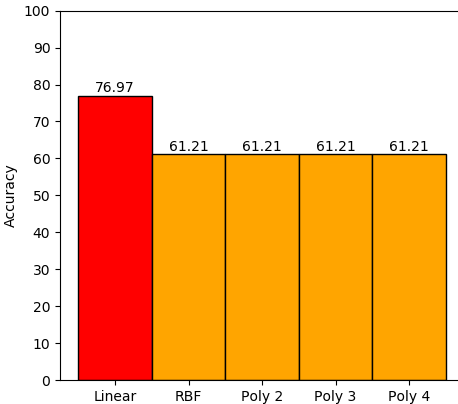
\includegraphics[width=0.8\linewidth]{SVM}
  \centering
  \caption{Evaluation on Support Vector Machine}
  \label{fig:SVM}
	\end{minipage}
	\begin{minipage}[t]{8.6cm}
	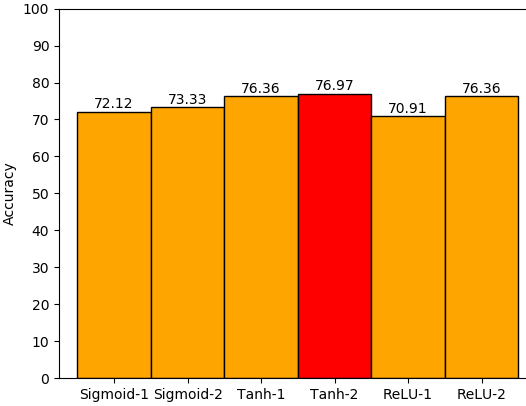
\includegraphics[width=0.92\linewidth]{MLP}
  \centering
  \caption{Evaluation on Multilayer Perceptron}
  \label{fig:MLP}
	\end{minipage}
\end{figure}

\begin{thebibliography}{1}
\bibitem{prostate} Ilir Agalliu, Robert Gern, Suzanne Leanza, and Robert D. Burk. 2009. {\em Associations of High-Grade Prostate Cancer with BRCA1 and BRCA2 Founder Mutations.} Clinical Cancer Research. Vol. 15, No. 3.
\bibitem{dnameth} Hao, Xiaoke, et al. {\em DNA methylation markers for diagnosis and prognosis of common cancers.} Proceedings of the National Academy of Sciences 114.28 (2017): 7414-7419.
\bibitem{praddata} Genome.ifmo.ru. (2018). TCGA PRAD Dataset. [online] Available at: {\em https://genome.ifmo.ru/files/software/phantasus/tcga/PRAD/ } [Accessed 29 Nov. 2018].
\bibitem{cosmicdata} Cancer.sanger.ac.uk. (2018). Cancer Gene Census. [online] Available at: {\em https://cancer.sanger.ac.uk/census } [Accessed 29 Nov. 2018].
\bibitem{civicdata} Civicdb.org. (2018). CIViC - Clinical Interpretations of Variants in Cancer. [online] Available at: {\em https://civicdb.org/releases } [Accessed 29 Nov. 2018].
\end{thebibliography}
\end{document}